\documentclass[12pt]{article}

\usepackage[a4paper,margin=1in]{geometry}
\usepackage{graphicx}
\usepackage{amsmath}
\usepackage{amssymb}
\usepackage{booktabs}
\usepackage{algorithm}
\usepackage{algpseudocode}
\usepackage{hyperref}
\usepackage{times}
\usepackage{tikz}
\usepackage{xcolor}
\usetikzlibrary{shapes.geometric, arrows.meta, positioning}
\usepackage{float}
\usepackage[skip=4pt]{caption}

\newcommand{\todo}[1]{\textcolor{blue}{\textbf{TODO:} #1}}

\setlength{\textfloatsep}{6pt plus 2pt minus 2pt}
\setlength{\intextsep}{6pt plus 2pt minus 2pt}
\setlength{\floatsep}{6pt plus 2pt minus 2pt}
\setlength{\abovecaptionskip}{3pt}
\setlength{\belowcaptionskip}{3pt}

\title{Distributed 3D Shape Classification\\ with a Quantized Embedded Convolutional Neural Network for Programmable Matter}
\author{Georges Chaiban \and Jad Bassil}
\date{July 2026}

\begin{document}

\maketitle
\begin{abstract}

\todo{Rewrite abstract: context, problem, novelty, results}

Programmable Matter (PM) systems are composed of many resource-constrained modules that must coordinate locally to sense, compute, and reconfigure without relying on centralized infrastructure. The core problem of PM is resource-constrained PM modules needing on-device shape recognition. Prior work proposed a 2D Artificial Neural Network (ANN), which does not scale to what is needed since it has high weight sizes for little configuration. This paper proposes an alternative and more efficient solution with the implementation of a 3D distributed Convolutional Neural Network (CNN) on a modular robot and PM system to detect shapes with different configurations. This also applies to fitting them into a real BlinkyBlocks platform, which requires further size limitations. The solution to that was to integrate TinyML with int8 quantization so that the model could be limited in size to fit within the hardware's flash memory. It was a necessary step because without it the model would not fit on the hardware at all. Our approach was then demonstrated both by simulation and by implementation on a real BlinkyBlocks platform. The conducted experimentation shows accuracies ranging from 73.3\% to 100\% per shape class, with an overall accuracy of 88.0\% on real hardware.

\end{abstract}

\section{Introduction}
\label{sec:introduction}


Programmable Matter (PM) can be defined as a modular robotic system of many identical modules that self-organize into different shapes and configurations. Each module is resource constrained in terms of memory and computational power, and can only communicate with its adjacent neighbors through local connections~\cite{Bourgeois2017}. Applications of PM include interactive CAD modeling~\cite{Bourgeois2017}, shape-shifting furniture~\cite{hauser2020roombots}, and self-assembling structures in space~\cite{postModularityFutureSpace2021}.

In all of these applications, the system has to know what shape it currently forms. A structure that recognizes it has become a chair can switch to the behavior expected from a chair, a reconfiguration process can check by itself that the target shape has been reached, and a CAD tool can be told which object the user has built. Recognizing the shape is difficult in PM, however: no module sees the whole configuration, there is no central coordinator, and each module has limited memory. The shape must therefore be recognized collectively, through local message passing between neighbors.

Earlier distributed algorithms, including our own~\cite{bassil2023shape,bassil2025configuration,bassil2026borderwalk}, solve part of this problem by recovering the \emph{geometry} of the configuration as a set of boxes or borders. They describe what the configuration looks like, but not what it is: assigning a class such as ``chair'' or ``bridge'' to the shape still needs an external computer. Piranda et al.~\cite{piranda2024ai4pm} took a first step toward on-device classification by mapping a distributed Artificial Neural Network (ANN) onto a grid of 256 modules arranged in a 2D grid, which recognized its own shape among three simple shapes (square, disk, triangle) with 552 bytes of memory per block. However, their approach handles 2D shapes only, and its fully-connected weights grow with the size of the grid, so larger or 3D configurations would need much more memory per block. It was also evaluated on only three simple shapes, each in a single fixed configuration.

In this paper, we address these limitations with a distributed 3D Convolutional Neural Network (CNN). Convolutions are local operations, so they map naturally onto the face-neighbor communication of lattice-based modules, and since the weights are shared across all modules, the memory needed per module does not depend on the size of the structure. The contributions of this paper are:
\begin{itemize}
  \item a distributed 3D CNN whose convolutions are computed through face-neighbor message passing, with the same weights shared by all modules so that the memory per module stays constant;
  \item a per-channel int8 weight quantization, following the TinyML approach~\cite{capogrosso}, that reduces the model size by 3.77 times to fit in BlinkyBlock flash memory, without changing the message format;
  \item an evaluation on six 3D shape classes in the VisibleSim simulator and on real BlinkyBlocks hardware, reaching 88.0\% overall accuracy, with per-class accuracy ranging from 73.3\% (Bridge) to 100\% (Sphere and Cylinder).
\end{itemize}

The rest of this paper is organized as follows. Section~\ref{sec:related_work} reviews related work. Section~\ref{sec:architecture} presents the distributed CNN architecture and its int8 quantization. Section~\ref{sec:experiments} reports the experimental setup and results. Section~\ref{sec:conclusion} concludes the paper.

\section{Related Work}
\label{sec:related_work}

Shape recognition in modular robots and PM systems has been studied from several angles. Early work framed it as a matching problem. Butler et al.~\cite{butler2002goal} proposed distributed algorithms that let modules decide whether the robot has reached a given goal configuration, and Shiu et al.~\cite{shiu2010graph} cast self-recognition as a graph isomorphism test between the connection graph of the robot and known configurations. Baca et al.~\cite{baca2015configuration} focused on discovering the configuration of a self-reconfigurable robot in real time, and Liu and Yim~\cite{liu2020configuration} showed how configurations can be recognized when the necessary information is distributed across the modules. These approaches work well for robots with tens of modules, but they usually rely on collecting the full connection graph, or compare it against a library of known configurations, which does not scale to PM systems made of hundreds or thousands of modules.

Our previous work tackled this scalability issue by computing a compact geometric description of the configuration directly inside the robot. In~\cite{bassil2023shape}, modules cooperate through message passing to find a set of overlapping boxes that cover the entire 3D configuration, so that the shape can be represented by a few boxes instead of the coordinates of every module. This box-search algorithm was then extended to react to module additions in real time, updating the description locally rather than running the whole algorithm again~\cite{bassil2025dynamic}. For 2D configurations, we replaced boxes with borders: modules search the internal and external borders of the configuration and share them so that each module can rebuild a global representation of the shape, which lowers communication cost compared to the box-based approach~\cite{bassil2025configuration}. BorderWalk~\cite{bassil2026borderwalk} then made border tracing fully distributed, with no central memory, by building communication bridges between borders through shortest-path spanning trees. All of these methods answer the question ``what does the configuration look like?'' by producing a geometric description. They do not answer ``what kind of object is it?'': assigning a semantic class to the shape (a chair, a bridge, a humanoid) still requires an external computer, or a hand-written rule for each class.

Learning-based methods address this second question. In Piranda et al.~\cite{piranda2024ai4pm} it is demonstrated that a shape-recognition ANN can be mapped as message-passing agents directly onto a BlinkyBlocks grid, and Dobreva et al.~\cite{dobreva} demonstrated separately that convolutional architectures using local, face-neighbor message passing can achieve direct distributed control on modular robots based on pivoting cubes. Combined, these results show that both fully-connected and convolutional models can be pushed down onto individual modules, and that convolution composes naturally with the face-adjacent communication pattern already native to these systems. We extend the distributed shape-recognition approach of Piranda et al.~\cite{piranda2024ai4pm} from a flat ANN over 2D silhouettes to a deeper, distributed 3D CNN for richer volumetric shapes.

Fitting a deeper model onto ressource-constrained hardware is more of a compression problem than anything else. Capogrosso et al.~\cite{capogrosso} review embedded-inference compression techniques, particularly post-training quantization (PTQ) and quantization-aware training (QAT), both of which reduce weight precision (usually to int8) to shrink the size of the model with limited accuracy loss. Somvanshi et al.~\cite{somvanshi} distinguish TinyML (inference on a single micro\-con\-trol\-ler-class device) from TinyDL (deeper models under the same resource envelope); our setting sits at the intersection of these two, since each module is itself a TinyML-class device, but the model as a whole is a deeper network distributed across many such devices. To the best of our knowledge, there is no previous work that integrates a distributed CNN, TinyML-style int8 quantization, and validation on real programmable-matter hardware as this paper does.

\section{Distributed 3D CNN Architecture}
\label{sec:architecture}

\subsection{System Model and Assumptions}
\label{sec:assumptions}
% While in Piranda et al.~\cite{piranda2024ai4pm} a shape was modeled as a 2D grid of lit and unlit points, the system presented here is based on a 3D grid of occupied and unoccupied cells. Our target shapes are volumetric: each module is placed in one cell of a 3D lattice, and the structure that is formed is a binary occupancy volume, where a cell is 1 if a BlinkyBlock is present at that position, and 0 otherwise. Each module then only ever needs to consider the local neighborhood of occupancy around its own position, rather than the shape as a whole, which is what makes a convolutional approach a natural fit: a 3D convolution is by definition a local operation over a neighborhood, and that neighborhood can be made to correspond exactly with the face-connections a BlinkyBlock physically has to its neighbors.

We consider a PM system made of $N$ BlinkyBlocks and make the following assumptions:
\begin{enumerate}
  \item \textbf{Lattice and shape representation.} Modules are cubes placed in the cells of a 3D cubic lattice. The shape is the binary occupancy volume of this lattice: a cell is 1 if a module occupies it and 0 otherwise. This extends the 2D grid of lit and unlit points used by Piranda et al.~\cite{piranda2024ai4pm} to volumetric shapes.
  \item \textbf{Connectivity.} The configuration is connected: every module can be reached from any other module through a chain of face-connected neighbors.
  \item \textbf{Local communication.} Each module has up to 6 face neighbors and can exchange messages only with them. Messages are asynchronous and are delivered reliably. There is no global clock and no global broadcast.
  \item \textbf{Local sensing.} Each module knows which of its faces are connected to a neighbor and can obtain the occupancy of its $3\times3\times3$ neighborhood with a one-message round trip. No module knows the whole configuration.
  \item \textbf{Identifiers.} Each module has a unique identifier. The module with $ID=1$ acts as the root of the spanning tree used for pooling and classification.
  \item \textbf{Static configuration.} The configuration does not change while the classification runs.
  \item \textbf{Homogeneous model.} All modules run the same program and store the same set of quantized weights, which must fit in the flash memory of a single module together with the firmware.
\end{enumerate}

Under these assumptions, each module only needs the occupancy around its own position, not the shape as a whole. This is what makes a convolutional approach a natural fit: a 3D convolution is a local operation over a neighborhood, and that neighborhood can be matched to the face connections each module physically has with its neighbors.

\subsection{Network Architecture}

\begin{figure}[tb]
    \centering
    \resizebox{!}{7.2cm}{
    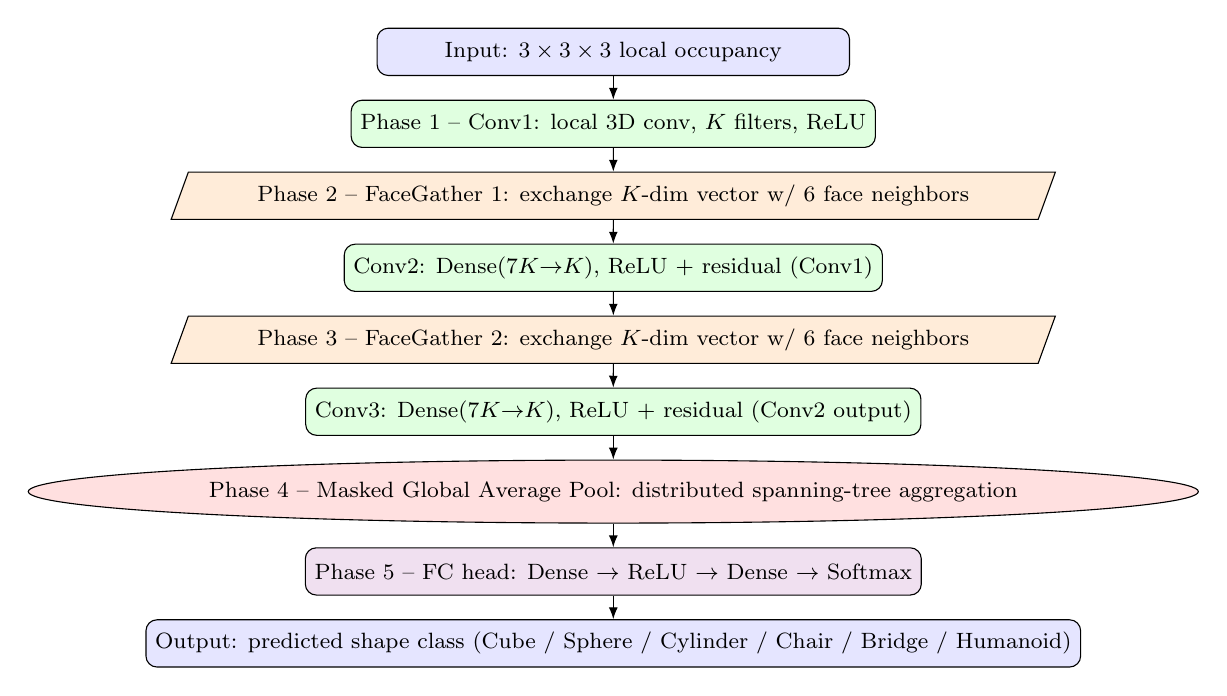
\begin{tikzpicture}[
        node distance=3mm,
        block/.style={rectangle, rounded corners, draw, fill=green!12, minimum width=6cm, minimum height=6mm, align=center, font=\footnotesize},
        msgblock/.style={trapezium, trapezium left angle=70, trapezium right angle=110, draw, fill=orange!15, minimum width=6cm, minimum height=6mm, align=center, font=\footnotesize},
        poolblock/.style={ellipse, draw, fill=red!12, minimum width=6cm, minimum height=8mm, align=center, font=\footnotesize},
        fcblock/.style={rectangle, rounded corners, draw, fill=violet!12, minimum width=6cm, minimum height=6mm, align=center, font=\footnotesize},
        ioblock/.style={rectangle, rounded corners, draw, fill=blue!10, minimum width=6cm, minimum height=6mm, align=center, font=\footnotesize},
        arr/.style={-{Latex[length=1.5mm]}}
    ]
        \node[ioblock] (input) {Input: $3\times3\times3$ local occupancy};
        \node[block, below=of input] (conv1) {Phase 1 -- Conv1: local 3D conv, $K$ filters, ReLU};
        \node[msgblock, below=of conv1] (fg1) {Phase 2 -- FaceGather 1: exchange $K$-dim vector w/ 6 face neighbors};
        \node[block, below=of fg1] (conv2) {Conv2: Dense($7K{\to}K$), ReLU + residual (Conv1)};
        \node[msgblock, below=of conv2] (fg2) {Phase 3 -- FaceGather 2: exchange $K$-dim vector w/ 6 face neighbors};
        \node[block, below=of fg2] (conv3) {Conv3: Dense($7K{\to}K$), ReLU + residual (Conv2 output)};
        \node[poolblock, below=of conv3] (pool) {Phase 4 -- Masked Global Average Pool: distributed spanning-tree aggregation};
        \node[fcblock, below=of pool] (fc) {Phase 5 -- FC head: Dense $\to$ ReLU $\to$ Dense $\to$ Softmax};
        \node[ioblock, below=of fc] (output) {Output: predicted shape class (Cube / Sphere / Cylinder / Chair / Bridge / Humanoid)};

        \draw[arr] (input) -- (conv1);
        \draw[arr] (conv1) -- (fg1);
        \draw[arr] (fg1) -- (conv2);
        \draw[arr] (conv2) -- (fg2);
        \draw[arr] (fg2) -- (conv3);
        \draw[arr] (conv3) -- (pool);
        \draw[arr] (pool) -- (fc);
        \draw[arr] (fc) -- (output);
    \end{tikzpicture}
    }
    \caption{Distributed 3D CNN architecture}
    \label{fig:architecture}
\end{figure}

The whole pipeline is illustrated in \figurename~\ref{fig:architecture}, which is divided into five phases performed sequentially by every module. The first convolution operator (Conv1) is computed directly by each block over its own $3\times3\times3$ occupancy neighborhood. The second and third phases are message-passed convolutions (Conv2, Conv3): each block exchanges its current $K$\-dimensional feature vector with its 6 face-connected neighbors, concatenates the 7 vectors, and passes the result through a dense layer with a residual connection, mirroring a convolution restricted to face-adjacent cells (diagonally adjacent neighbors are not reachable in a single message hop). Each stage adds one more hop of face-neighbor context to the effective receptive field. Phase 4 performs masked global average pooling, distributed along a spanning tree. In Phase 5, a two-layer fully connected head produces a 6-way softmax over the shape classes.

The features become more global from one phase to the next. After Conv1, a module's features describe the local geometry around it, for example whether it lies inside the volume, on a flat face, along an edge, at a corner, or in a structure only one module thick. Each message-passed convolution widens this view by one hop, so after Conv3 the features capture larger parts of the shape, such as pillars, flat plates, or curved surfaces. Global pooling then summarizes how often these parts appear across the whole structure, which is what the classifier uses to tell the shapes apart. Since all modules share the same weights, the same features are computed anywhere in the structure, regardless of the size and position of the shape.



To summarize, the recognition process applies the following equations at each block. Let $V_{i,j,k}$ denote the block's local $3\times3\times3$ occupancy window ($i,j,k \in \{0,1,2\}$), and let $K$ be the number of feature channels per block.

\textbf{Phase 1 (Conv1, local, no messages):}
\begin{equation}
\text{Conv1}_f = \mathrm{ReLU}\left(b^{(1)}_f + \sum_{i,j,k=0}^{2} W^{(1)}_{f,i,j,k} \cdot V_{i,j,k}\right), \quad f = 1,\dots,K
\label{eq:conv1}
\end{equation}

\textbf{Phase 2 (Conv2, message-passed, 1 hop):} each block concatenates its own Conv1 output with the Conv1 outputs received from its 6 face neighbors into a $7K$-dimensional vector $X^{(2)}$, then applies:
\begin{equation}
\text{Conv2}_f = \mathrm{ReLU}\left(b^{(2)}_f + \sum_{i=1}^{7K} W^{(2)}_{f,i} \cdot X^{(2)}_i\right), \qquad H^{(2)}_f = \text{Conv2}_f + \text{Conv1}_f
\label{eq:conv2}
\end{equation}

\textbf{Phase 3 (Conv3, message-passed, 2nd hop):} identical in form to Phase 2, but built from $H^{(2)}$ instead of Conv1, giving a $7K$-dimensional $X^{(3)}$:
\begin{equation}
\text{Conv3}_f = \mathrm{ReLU}\left(b^{(3)}_f + \sum_{i=1}^{7K} W^{(3)}_{f,i} \cdot X^{(3)}_i\right), \qquad H^{(3)}_f = \text{Conv3}_f + H^{(2)}_f
\label{eq:conv3}
\end{equation}

\textbf{Phase 4 (distributed pooling):} the structure's total feature sum $S$ and occupied-block count $N$ are aggregated over a spanning tree rooted at one block, then averaged:
\begin{equation}
S = \sum_{\text{occupied blocks}} H^{(3)}, \qquad N = \sum_{\text{occupied blocks}} 1, \qquad A = S / N
\label{eq:pool}
\end{equation}

\textbf{Phase 5 (classification head, root only):}
\begin{equation}
Z = \mathrm{ReLU}(W^{(fc1)} A + b^{(fc1)}), \qquad P = \mathrm{Softmax}(W^{(fc2)} Z + b^{(fc2)})
\label{eq:fc}
\end{equation}

Each receiving block must be aware once it has received a message from all of its face neighbors, since a message that will never arrive (e.g. from a boundary face with no neighbor) must not be waited on forever. This can be easily checked by each block counting the number of face neighbors it has, and marking each neighbor as ``reported'' when a message is received from it. Once all neighbors have reported, the block can proceed to the next phase.

% For this purpose we introduce three agents to map these phases onto BlinkyBlocks messages, shown in Algorithms~\ref{alg:phase1}--\ref{alg:phase45}.

\begin{algorithm}[tb]
\caption{Phase 1: Local Feature Extraction (Conv1)}
\label{alg:phase1}
\begin{algorithmic}[1]
\Function{Startup}{}
    \State $V \gets \Call{QueryNeighborhood}{}$ \Comment{$3\times3\times3$ local occupancy scan}
    \For{$f \gets 1$ \textbf{to} $K$}
        \State $sum \gets b^{(1)}_f + \sum_{i,j,k} V_{i,j,k} \times W^{(1)}_{f,i,j,k}$
        \State $\text{Conv1}_f \gets \max(0, sum)$
    \EndFor
    \If{$ID = 1$}
        \State \Call{InitiateSpanningTree}{}
    \EndIf
    \State \Call{Broadcast}{Conv1} to face-neighbors
\EndFunction
\end{algorithmic}
\end{algorithm}

\begin{algorithm}[tb]
\caption{Phases 2/3: Message-Passed Convolution (Conv2, Conv3)}
\label{alg:phase23}
\begin{algorithmic}[1]
\Function{HandleFeatureMsg}{msg}
    \State Save received feature vector from neighbor to memory
    \If{all face neighbors reported}
        \State $X \gets [H_{self}, H_{n_1}, \dots, H_{n_6}]$ \Comment{$7K$-dim concatenation}
        \For{$f \gets 1$ \textbf{to} $K$}
            \State $sum \gets b_f + \sum_i X_i \times W_{f,i}$
            \State $\text{Conv}_f \gets \max(0, sum) + H_{self,f}$ \Comment{residual add}
        \EndFor
        \State \Call{CheckReadyToAggregate}{} \Comment{See Algorithm~\ref{alg:phase45}}
    \EndIf
\EndFunction
\end{algorithmic}
\end{algorithm}

\begin{algorithm}[tb]
\caption{Phases 4/5: Distributed Aggregation and Classification}
\label{alg:phase45}
\begin{algorithmic}[1]

\Function{CheckReadyToAggregate()}{}
    \If{Conv3 done \textbf{and} tree built \textbf{and} all children done}
        \State $S \gets H^{(3)}_{self} + \sum_{c \in children} S_{child}[c]$ \Comment{feature sum of own subtree}
        \State $N \gets 1 + \sum_{c \in children} N_{child}[c]$ \Comment{module count of own subtree}
        \If{$self$ is Root}
            \State $A \gets S / N$ \Comment{global average, Eq.~\ref{eq:pool}}
            \State \Call{Classify}{$A$} \Comment{Eq.~\ref{eq:fc}}
        \Else
            \State \Call{Send}{\textsc{Aggregate}$(self, S, N)$} to $parent$ \Comment{handled by \textsc{HandleAggregateMsg}}
        \EndIf
    \EndIf
\EndFunction
\Statex
\Function{HandleAggregateMsg}{$c, S_c, N_c$} \Comment{received from child $c$}
    \State $S_{child}[c] \gets S_c$; \quad $N_{child}[c] \gets N_c$ \Comment{partial sum and count of $c$'s subtree}
    \State mark child $c$ as done
    \State \Call{CheckReadyToAggregate()}{}
\EndFunction
\end{algorithmic}
\end{algorithm}


Algorithms~\ref{alg:phase1}--\ref{alg:phase45} describe the distributed execution of the five phases. Each module runs the same code, and the phases are executed sequentially. The first phase is local, so no messages are sent. In Phases 2 and 3, each module sends its current feature vector to its face neighbors and waits until it has received a feature vector from all of them before proceeding. Phase 4 aggregates the features along a spanning tree rooted at one module, which is built in parallel with the convolutions. Each module waits until it has received an aggregate message from all of its children before sending its own aggregate to its parent. The root computes the global average and passes it through the classification head. It can then broadcast the predicted class to all modules if desired, but this is not necessary for the classification itself.


\subsection{Message Passing and Complexity}
\label{sec:complexity}

Each module can only communicate with its directly face-connected neighbors; there is no global broadcast. We analyze the communication cost of each step for a configuration of $N$ modules connected by $E$ face-to-face links. Since a module has at most 6 neighbors, $E \le 3N$. We denote by $D$ the eccentricity of the root, that is, the largest number of hops between the root and any other module ($D \le N-1$).

\paragraph{Spanning tree.} The tree is built by flooding from the root: when a module receives the construction message for the first time, it takes the sender as its parent and forwards the message to its other neighbors, and every module then tells its parent whether it accepted it as a child. Each link therefore carries a constant number of messages in each direction, for a total of $O(E) = O(N)$ messages, and the construction completes in $O(D)$ communication rounds.

\paragraph{Local features.} Before Conv1, each module sends a single message to each of its face neighbors, containing a 6-bit mask of its own connected faces. From the masks it receives, a module rebuilds its $3\times3\times3$ occupancy neighborhood, including the diagonal cells it cannot sense directly, and then computes Conv1 locally. This exchange costs $2E \le 6N$ messages and one round. In each of the two message-passed convolutions (Conv2 and Conv3), every module sends one $K$-dimensional feature vector to each of its face neighbors, so each phase uses exactly $2E \le 6N$ messages and completes in a single round, whatever the shape. Together, the three exchanges cost $6E \le 18N$ messages.

\paragraph{Aggregation.} During pooling, every module except the root sends exactly one \textsc{Aggregate} message, carrying the feature sum ($K$ values) and module count of its subtree, to its parent. Aggregation thus uses $N-1$ messages and completes in $D$ rounds, since a module can only report once all of its children have reported.

Overall, a full classification uses $O(E) = O(N)$ messages, at most a constant number per module, and completes in $O(D)$ rounds. Since the convolution phases take a constant number of rounds, the running time is dominated by building the tree and aggregating along it, which depends on the diameter of the configuration rather than on its complexity. Because each block only keeps its own weights and a small, fixed number of feature vectors, the memory required per module is $O(1)$ with respect to the total number of modules in the system.

\subsection{Training}
\label{sec:training}

The network is trained offline, on a workstation, and only inference runs on the modules. For training, we write the distributed network as an equivalent centralized model in TensorFlow/Keras that operates on the full occupancy grid. Conv1 is a standard $3\times3\times3$ convolution with $K$ filters. Conv2 and Conv3 are convolutions whose kernel is restricted to the center cell and its 6 face neighbors, which is exactly what each module computes from its own feature vector and those received from its neighbors (Eqs.~\ref{eq:conv2} and~\ref{eq:conv3}). After each layer, the features of empty cells are set to zero, so that empty cells contribute nothing, just as a missing neighbor sends no message. The pooling layer averages the features over occupied cells only (Eq.~\ref{eq:pool}), and the classification head is the same two-layer network as in Eq.~\ref{eq:fc}. Because the centralized model and the distributed one compute the same function, the trained weights can be copied directly to the modules, and every module stores the same set of weights.

\textbf{Dataset.} We generate the training data procedurally. Each sample is a $16\times16\times16$ binary occupancy grid containing one shape from one of six classes: Cube, Sphere, Cylinder, Chair, Bridge, and Humanoid. Shapes are built from simple primitives (boxes, spheres, cylinders, and limbs for the humanoid), and their dimensions and position are drawn at random for every sample. To cover the conditions met on real structures, each class mixes several variants: axis-aligned shapes, shapes rotated by three random Euler angles, very small shapes, and ``overflowing'' shapes that are larger than the grid and therefore only partially visible. The humanoid is generated with random joint angles for the arms and legs, so that it appears in many different postures. Each sample is also mirrored along each axis with probability 0.5, which makes the model insensitive to the handedness of the hardware coordinate system, and samples with fewer than 6 occupied cells or more than 97\% occupancy are discarded. Finally, 1\% of the cells of each training sample are set to 1 at random, to make the model robust to sensing errors; this noise is not added to the validation and test sets. The training set contains 60{,}000 samples (10{,}000 per class), and separate validation and test sets of 6{,}000 and 3{,}000 samples are generated with fixed random seeds.

\textbf{Optimization.} We use $K=32$ feature channels and a hidden layer of 48 neurons in the classification head, which gives 17{,}174 parameters in total. The model is trained in float32 with a categorical cross-entropy loss, using the Adam optimizer with gradient-norm clipping at 1.0 and a batch size of 128. The learning rate rises linearly to $10^{-3}$ during the first 10 epochs, then follows a cosine decay down to $10^{-6}$. Dropout with rate 0.3 is applied after the hidden layer of the head during training only. Training runs for up to 200 epochs, with early stopping when the validation accuracy has not improved for 30 epochs, after which the best weights are restored. Once training has finished, the weights and biases are exported as a C header file that is compiled into the firmware. Quantization is applied afterward, to this exported model, without any retraining (Section~\ref{sec:quantization}).

\subsection{TinyML Int8 Quantization}
\label{sec:quantization}

\begin{figure}[tb]
    \centering
    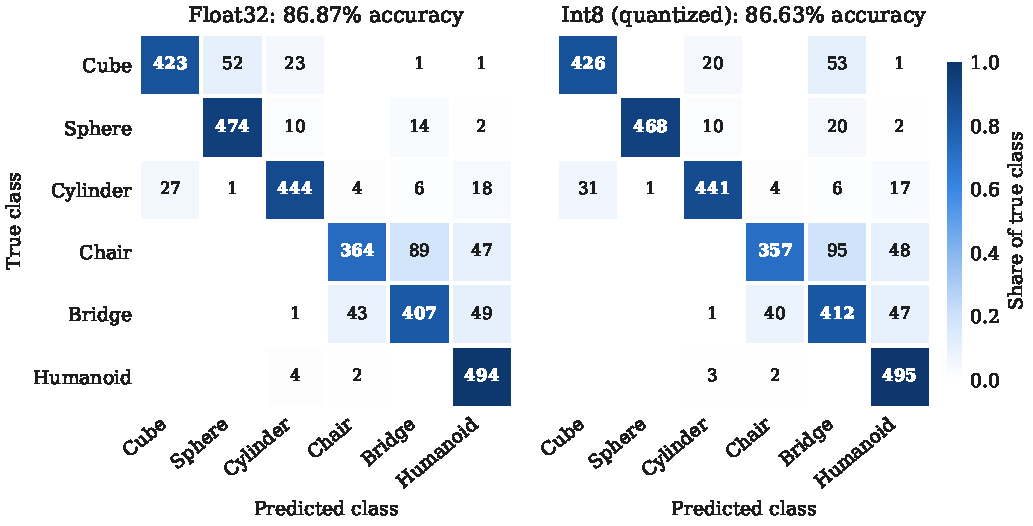
\includegraphics[width=\textwidth]{figures/AI4PM-CNN/AI4PM-DeepEmbedded/quantization_confusion.pdf}
    \caption{Confusion matrices of the float32 (left) and int8 (right) models on 3{,}000 generated test shapes (500 per class). Rows are true classes and columns predicted classes; cells give counts, shaded by their share of the true class.}
    \label{fig:quantization}
\end{figure}

Although the number of parameters in the trained float32 model was small, it was still too large to fit in BlinkyBlock flash memory once weights, biases, and firmware were accounted for. We applied weight-only int8 post-training quantization~\cite{capogrosso} to the five weight tensors. Each output channel $c$ (a convolution filter or an output neuron of a dense layer) gets its own symmetric scale $s_c = \max_i |w_{c,i}| / 127$, and each weight is stored as $q_{c,i} = \mathrm{clip}(\mathrm{round}(w_{c,i}/s_c), -127, 127)$. Biases and activations remain float32, so the messages exchanged between modules are unchanged. At inference, a module computes each output as $y_c = s_c \sum_i q_{c,i}\, x_i + b_c$, multiplying by the scale once per output rather than once per weight. The model stores 17{,}024 int8 weights, plus 150 float32 biases and 150 float32 scales, for a total of 17.8~KB instead of 67.1~KB in float32, a 3.77x reduction.

To measure the cost of quantization, we ran the trained network with the float32 weights and with the dequantized int8 weights on the same 3{,}000 shapes, generated by the training generator without noise (500 per class). Accuracy drops from 86.87\% to 86.63\%, and the two models give the same prediction for 97.3\% of the shapes. \figurename~\ref{fig:quantization} shows the confusion matrices of both models: the per-class accuracy changes by at most 1.4 points (Chair, from 72.8\% to 71.4\%), and no class collapses into another. Most of the disagreements are Cube samples that both models misclassify, which float32 predicts as Sphere and int8 as Bridge.

\section{Experiments and Results}
\label{sec:experiments}

\todo{Rewrite}
\subsection{Experimental Setup}
\label{sec:setup}

% We created a synthetic training set of six classes of 3D shapes (Cube, Sphere, Cylinder, Chair, Bridge, Humanoid), randomly sized, positioned, and oriented per sample procedurally so the model would not overfit to a single fixed pose. The model was trained on these ground-truth occupancy grids and exported to the quantized int8 header of Section~\ref{sec:quantization}, then evaluated in VisibleSim~\cite{piranda2024ai4pm} and on real BlinkyBlocks hardware. For the real-hardware evaluation we swept shape size, rotation, translation, and non-uniform scaling per class, including out-of-distribution configurations, to test generalization beyond the training conditions.

We evaluated the model in VisibleSim~\cite{piranda2024ai4pm}, which runs the same distributed algorithm as the BlinkyBlocks firmware, with the float32 weights, and on real BlinkyBlocks with the int8 weights (Section~\ref{sec:quantization}).

\paragraph{Simulation.} The sweep contains 100 configurations (20 Cube, 20 Sphere, 20 Cylinder, 15 Chair, 15 Bridge, 10 Humanoid) that vary size, rotation, translation, and scaling, including sizes outside the training range and chair variants absent from the training generator (armrests, thin legs, tall back). Bridges and humanoids are built with the training generator in a $16\times16\times16$ grid; the other classes are placed in a $50\times50\times50$ lattice, so the structures range from 18 to 33{,}401 modules (median 387).

\paragraph{Hardware.} We ran the quantized firmware on physical BlinkyBlocks for all six classes, varying the size, rotation, translation, and scale of the shapes. \todo{number of configurations per class, number of modules per structure, and how each configuration was assembled}

\subsection{Simulation Results}
\begin{table}[tb]
    \centering
    \caption{VisibleSim simulation results (float32 weights), one representative instance per class.}
    \label{tab:sim-results}
    \small
    \begin{tabular}{lccccc}
        \toprule
        Shape & Predicted & Confidence & Blocks & Messages & Bandwidth \\
        \midrule
        Cube     & Cube     & 100.0\% & 125 & 2{,}152 & 129{,}856 B \\
        Sphere   & Sphere   & 100.0\% & 33  & 416     & 26{,}648 B \\
        Cylinder & Cylinder & 100.0\% & 261 & 4{,}504 & 271{,}872 B \\
        Chair    & Chair    & 100.0\% & 61  & 616     & 41{,}888 B \\
        Bridge   & Bridge   & 100.0\% & 57  & 624     & 41{,}512 B \\
        Humanoid & Humanoid & 100.0\% & 54  & 590     & 39{,}260 B \\
        \bottomrule
    \end{tabular}
\end{table}

\begin{table}[tb]
    \centering
    \caption{VisibleSim classification accuracy over the 100-configuration sweep (float32 weights).}
    \label{tab:sim-sweep}
    \begin{tabular}{lccl}
        \toprule
        Shape & Correct / Total & Accuracy & Misclassified as \\
        \midrule
        Cube      & 13/20 & 65.0\%  & Cylinder (5), Bridge (2) \\
        Sphere    & 20/20 & 100.0\% & -- \\
        Cylinder  & 17/20 & 85.0\%  & Sphere (2), Cube (1) \\
        Chair     & 13/15 & 86.7\%  & Cylinder (1), Bridge (1) \\
        Bridge    & 15/15 & 100.0\% & -- \\
        Humanoid  & 10/10 & 100.0\% & -- \\
        \midrule
        Overall   & 88/100 & 88.0\% & \\
        \bottomrule
    \end{tabular}
\end{table}

Table~\ref{tab:sim-results} gives one instance per class: all six are recognized with 100.0\% confidence, and messages and bandwidth grow with the number of modules (Section~\ref{sec:complexity}). Over the full sweep (Table~\ref{tab:sim-sweep}), the model classifies 88 of the 100 configurations correctly, and Sphere, Bridge, and Humanoid are always recognized. Eight of the 12 errors are Cubes and Cylinders rotated by arbitrary angles, whose jagged voxelized boundary resembles a curved surface. The others are a flat box and a thin-legged chair taken for Bridges, a very large rotated chair (4{,}687 modules) taken for a Cylinder, and a rotated cube that voxelizes into pieces that are not face-connected, of which only the piece containing the root is aggregated. \figurename~\ref{fig:sim-shapes} shows the six instances in VisibleSim.

\begin{figure}[tb]
    \centering
    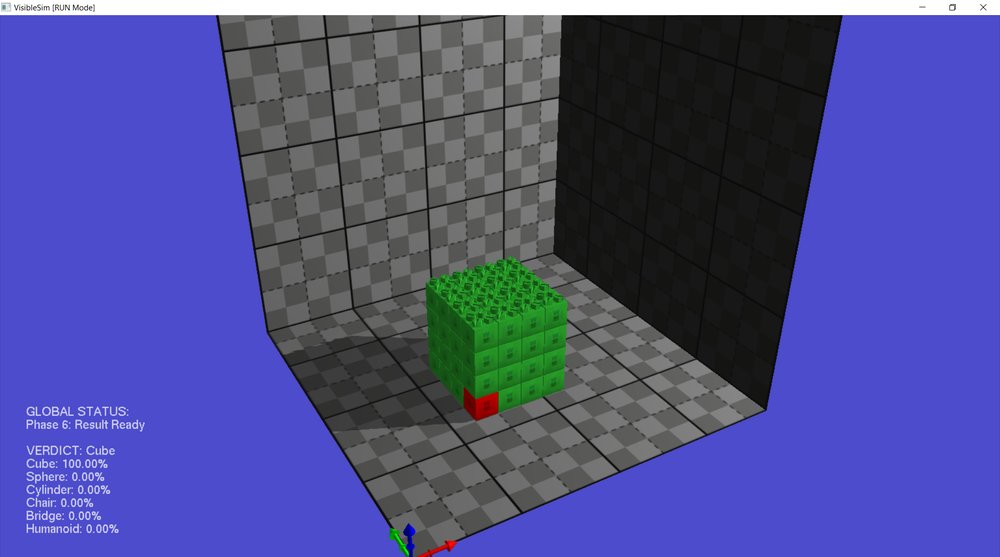
\includegraphics[width=0.3\textwidth]{figures/AI4PM-CNN/AI4PM-DeepEmbedded/sim_cube.png}
    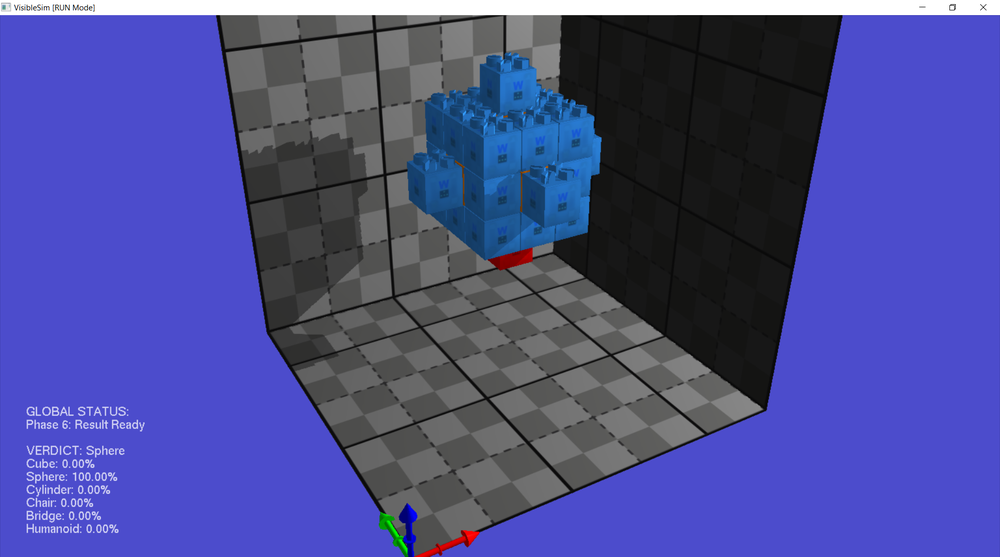
\includegraphics[width=0.3\textwidth]{figures/AI4PM-CNN/AI4PM-DeepEmbedded/sim_sphere.png}
    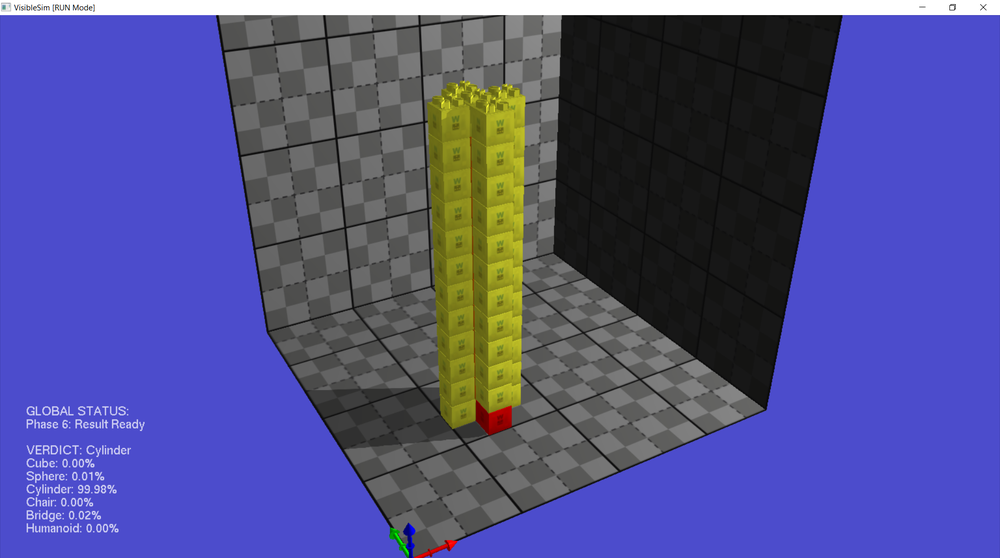
\includegraphics[width=0.3\textwidth]{figures/AI4PM-CNN/AI4PM-DeepEmbedded/sim_cylinder.png}\\[2mm]
    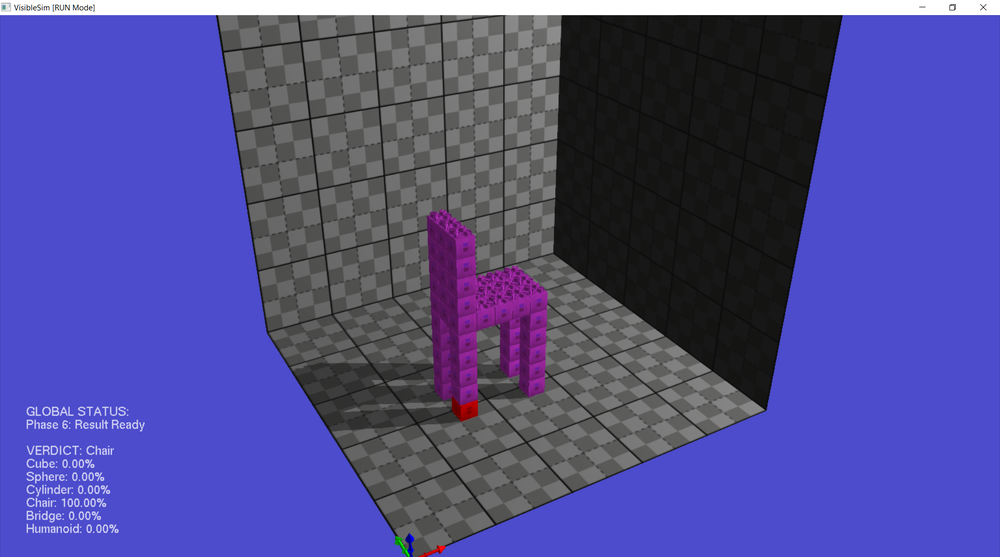
\includegraphics[width=0.3\textwidth]{figures/AI4PM-CNN/AI4PM-DeepEmbedded/sim_chair.png}
    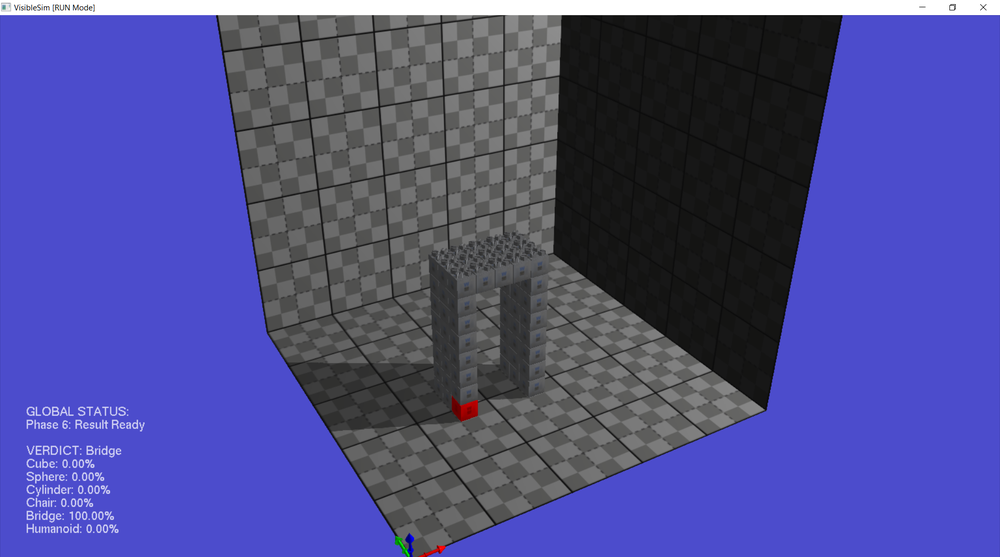
\includegraphics[width=0.3\textwidth]{figures/AI4PM-CNN/AI4PM-DeepEmbedded/sim_bridge.png}
    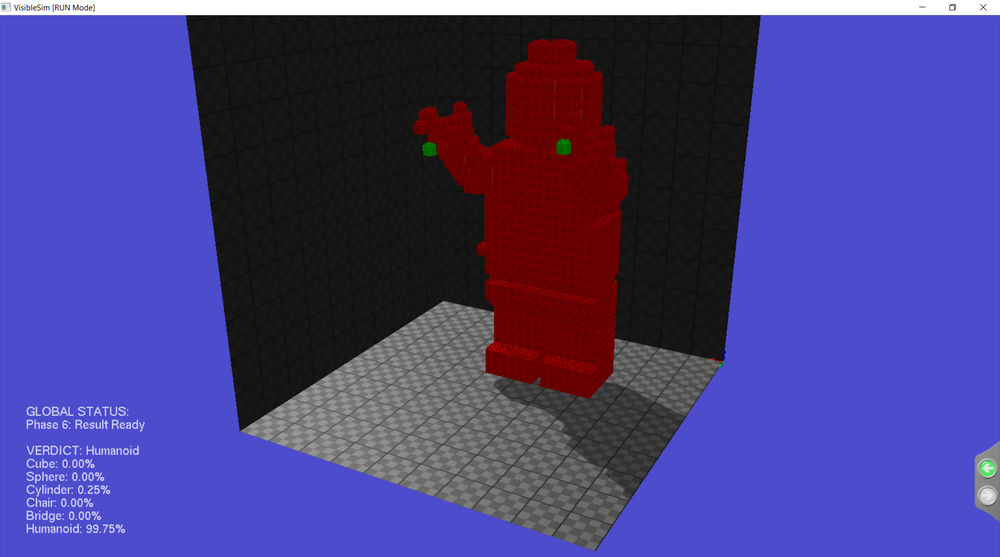
\includegraphics[width=0.3\textwidth]{figures/AI4PM-CNN/AI4PM-DeepEmbedded/sim_humanoid.png}
    \caption{VisibleSim classification results for all six shape classes. Top row, left to right: Cube, Sphere, Cylinder. Bottom row: Chair, Bridge, Humanoid.}
    \label{fig:sim-shapes}
\end{figure}

\subsection{Hardware Results}

\begin{table}[tb]
    \centering
    \caption{Real BlinkyBlocks hardware classification accuracy by shape (quantized model).}
    \label{tab:hw-results}
    \begin{tabular}{lcc}
        \toprule
        Shape & Correct / Total & Accuracy \\
        \midrule
        Cube      & 17/20 & 85.0\% \\
        Sphere    & 20/20 & 100.0\% \\
        Cylinder  & 20/20 & 100.0\% \\
        Chair     & 12/15 & 80.0\% \\
        Bridge    & 11/15 & 73.3\% \\
        Humanoid  & 8/10  & 80.0\% \\
        \midrule
        Overall   & 88/100 & 88.0\% \\
        \bottomrule
    \end{tabular}
\end{table}

On hardware (Table~\ref{tab:hw-results} and \figurename~\ref{fig:accuracy-hw}), the model reaches 88.0\% overall: Sphere and Cylinder are always recognized, Cube reaches 85.0\%, Chair and Humanoid 80.0\%, and Bridge is the weakest class at 73.3\%. \figurename~\ref{fig:hardware-photos} shows four classified structures.

\begin{figure}[tb]
    \centering
    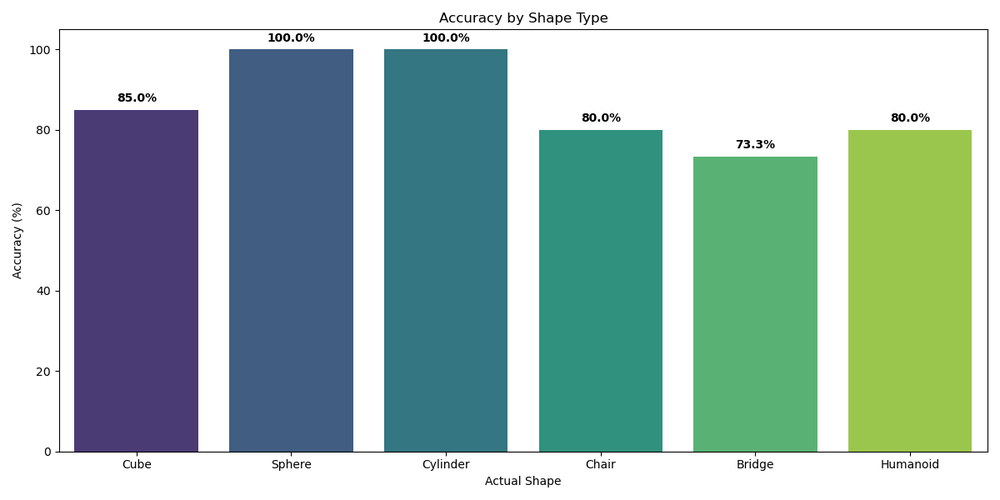
\includegraphics[width=0.8\textwidth]{figures/AI4PM-CNN/AI4PM-DeepEmbedded/hw_accuracy_by_shape.png}
    \caption{Per-class classification accuracy of the quantized 3D CNN model.}
    \label{fig:accuracy-hw}
\end{figure}

\begin{figure}[tb]
    \centering
    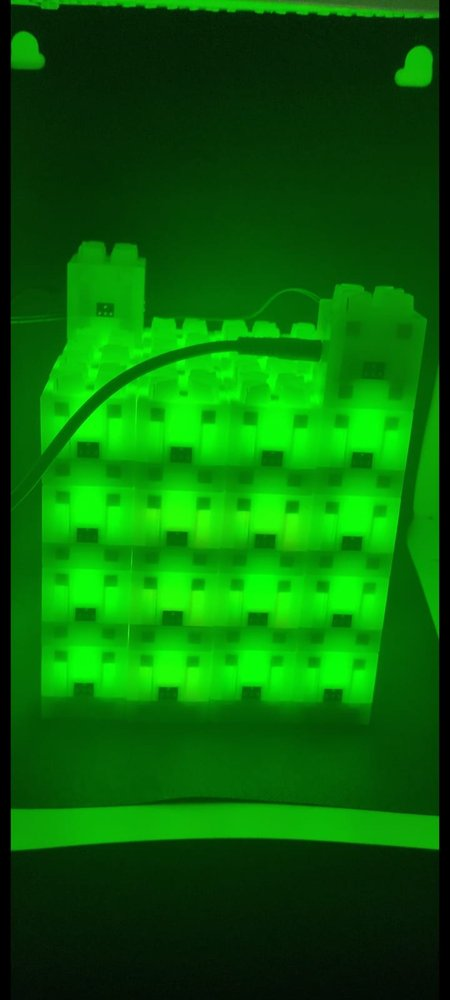
\includegraphics[height=4.5cm,keepaspectratio]{figures/AI4PM-CNN/AI4PM-DeepEmbedded/hw_cube.jpeg}
    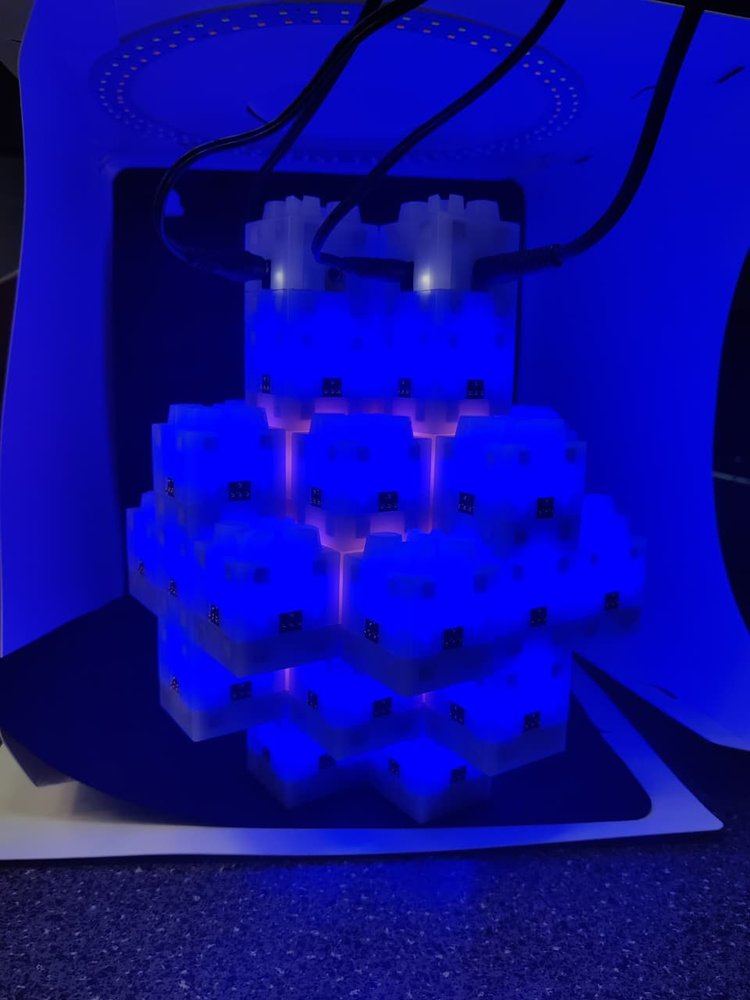
\includegraphics[height=4.5cm,keepaspectratio]{figures/AI4PM-CNN/AI4PM-DeepEmbedded/hw_sphere.jpeg}
    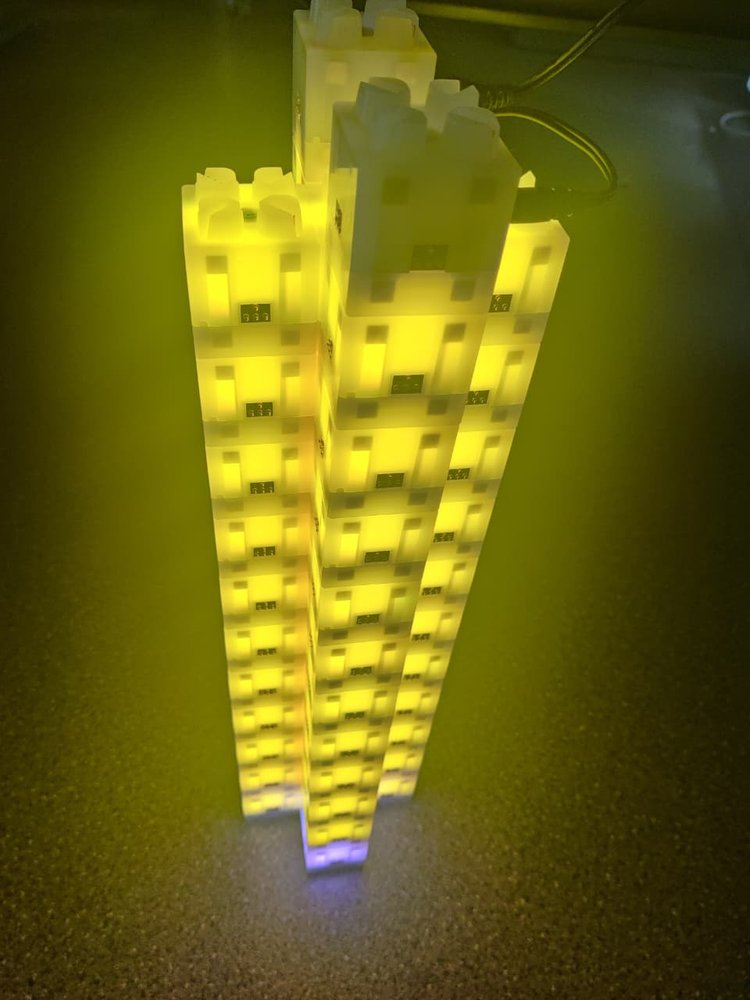
\includegraphics[height=4.5cm,keepaspectratio]{figures/AI4PM-CNN/AI4PM-DeepEmbedded/hw_cylinder.jpeg}
    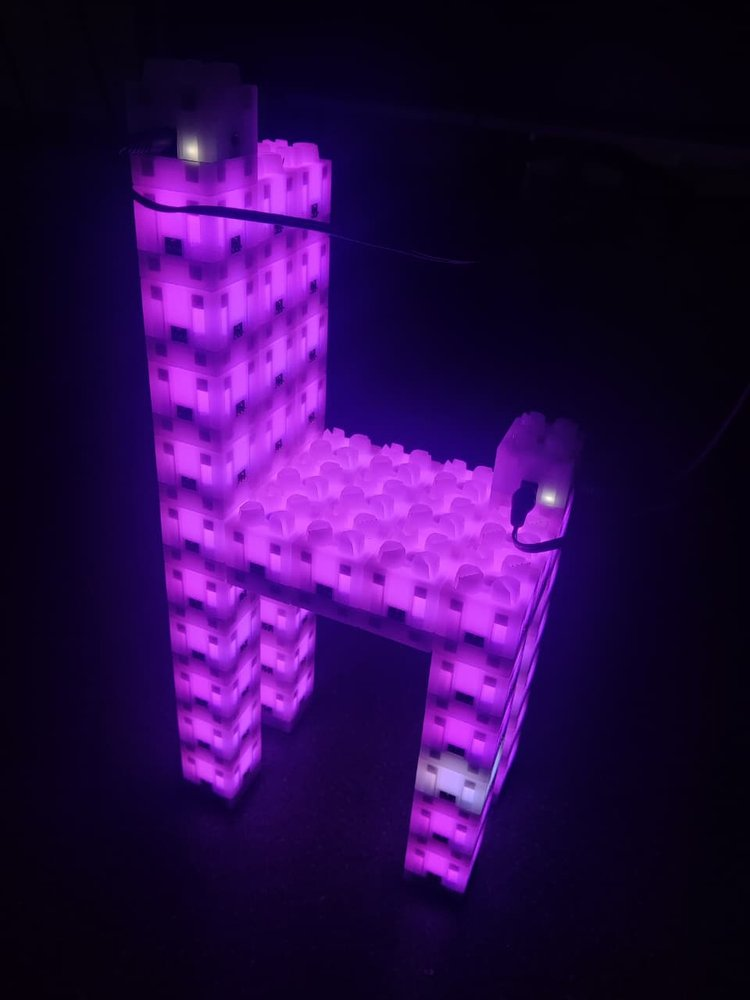
\includegraphics[height=4.5cm,keepaspectratio]{figures/AI4PM-CNN/AI4PM-DeepEmbedded/hw_chair.jpeg}
    \caption{Real BlinkyBlocks running the distributed 3D CNN classifier. Modules light up in the color of the predicted class (Cube: green, Sphere: blue, Cylinder: yellow, Chair: magenta).}
    \label{fig:hardware-photos}
\end{figure}

\subsection{Discussion}

Both evaluations reach 88.0\%, but the errors differ: in simulation they come mostly from arbitrarily rotated Cubes and Cylinders, and on hardware from the classes with parts one module thick (Bridge, Chair, Humanoid). We attribute this shift to how the $3\times3\times3$ window is obtained. VisibleSim reads the 26 surrounding cells directly from the lattice, whereas a hardware module senses only its 6 face neighbors and rebuilds the other 20 cells from their connectivity masks (Section~\ref{sec:complexity}): an edge cell is detected if one of its two adjacent face neighbors is present, and a corner cell by a majority vote over its three adjacent edge cells. These rules are exact inside a solid volume but can fail where the structure is one module thick, and the resulting errors in Conv1 then spread through Conv2 and Conv3.

Communication follows the analysis of Section~\ref{sec:complexity}: across the sweep, each module sends 9 to 21 messages for structures of 18 to 33{,}401 modules, and uses the same memory in every run (about 2.8~KB of buffers for $K=32$, plus the shared weights). The cost of classification thus depends on the size of the structure, not on the complexity of its shape.

Compared with Piranda et al.~\cite{piranda2024ai4pm}, who classified three 2D shapes in one fixed configuration each, our model handles six 3D classes under changes of size, position, orientation, and scale, within the flash memory of a single module. With 10 to 20 configurations per class, the per-class figures are only indicative. Moreover, the simulation uses float32 weights and the hardware int8 weights; since quantization costs only 0.23 points on generated shapes (Section~\ref{sec:quantization}), occupancy reconstruction likely explains most of the difference, although this was not measured on the 100 configurations. Running the float32 model on hardware and training on reconstructed occupancy windows are natural next steps.

\section{Conclusion}
\label{sec:conclusion}

In this paper, a distributed 3D Convolutional Neural Network for module shape classification on Programmable Matter systems is presented. It shows that a deep learning model can be distributed across a modular robotic system, with each module computing its own local features and exchanging messages with its neighbors to build a global understanding of the shape. The model is trained offline and then quantized to fit within the memory constraints of the modules, achieving high accuracy in both simulation and real hardware tests. To fit the model within the flash memory budget of a BlinkyBlock, we applied TinyML weight quantization, converting the trained weights from float32 to int8 and reducing model size by 3.77 times with no change to the message format. We validated the model both in simulation and on a real modular robot platform, getting an overall accuracy of 88.0\% across all six classes in both cases. On hardware, per-class accuracy ranged from 73.3\% (Bridge) to 100\% (Sphere and Cylinder); in simulation, from 65.0\% (Cube, mostly under arbitrary rotations) to 100\% (Sphere, Bridge, and Humanoid). Thin shapes like the Bridge remain the hardest case, since a real BlinkyBlock can only directly sense its 6 face-connected neighbors, so closing this gap, alongside expanding the shape classes and testing on larger real configurations, is left as future work.

\section*{Acknowledgment}

\bibliographystyle{IEEEtran}
\bibliography{bibliography}

\end{document}
